\section{Class Description}

\subsection{Authentication}
\subsubsection{App}
\label{App}
\begin{wrapfigure}{l}{4.5cm}
    \raisebox{0pt}[\dimexpr\height-0.5\baselineskip\relax]{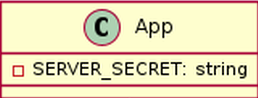
\includegraphics[width=4.5cm]{classes/auth/app.png}}
\end{wrapfigure} 
\par
The main class of the authentication service.
\newline
\newline
\textbf{Attributes}
\begin{itemize}
    \item \textbf{SERVER\_SECRET} the encryption key that is shared among all the services to decrypt tokens
\end{itemize}

\subsubsection{UserModel}
\label{UserModel}
\begin{wrapfigure}{l}{4.5cm}
    \raisebox{0pt}[\dimexpr\height-0.5\baselineskip\relax]{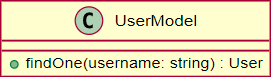
\includegraphics[width=4.5cm]{classes/auth/1.png}}
\end{wrapfigure} 
\par
The collection of registered users in the database.
\newline
\newline
\textbf{Methods}
\begin{itemize}
    \item \textbf{findOne} returns the user that has the matching username
\end{itemize}

\subsubsection{User}
\label{User}
\begin{wrapfigure}{l}{4.5cm}
    \raisebox{0pt}[\dimexpr\height-0.5\baselineskip\relax]{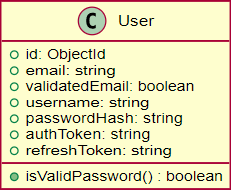
\includegraphics[width=4.5cm]{classes/auth/2.png}}
\end{wrapfigure} 
\par
A registered user
\newline
\newline
\textbf{Attributes}
\begin{itemize}
    \item \textbf{email} email of the user
    \item \textbf{validatedEmail} iff the email is validated
    \item \textbf{username} username of the user
    \item \textbf{passwordHash} hash of the password of the user
    \item \textbf{authToken} the current authentication token of the user
    \item \textbf{refreshToken} the current refresh token of the user
\end{itemize}
\textbf{Methods}
\begin{itemize}
    \item \textbf{isValidPassword} iff the supplied password is valid
\end{itemize}

\subsubsection{EmailValidator}
\label{EmailValidator}
\begin{wrapfigure}{l}{4.5cm}
    \raisebox{0pt}[\dimexpr\height-0.5\baselineskip\relax]{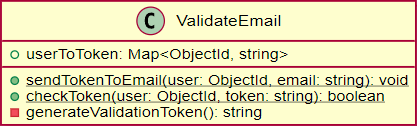
\includegraphics[width=4.5cm]{classes/auth/3.png}}
\end{wrapfigure} 
\par
This static class sends an email to the user with a token and checks if the given token is correct.
\newline
\newline
\textbf{Attributes}
\begin{itemize}
    \item \textbf{userToToken} maps the user id to the sent token
\end{itemize}
\textbf{Methods}
\begin{itemize}
    \item \textbf{sendTokenToEmail} sends a token to the given email 
    \item \textbf{checkToken} compares the received token with the token sent to email
    \item \textbf{generateValidationToken} generates a validation token
\end{itemize}

\subsubsection{TokenContent}
\label{TokenContent}
\begin{wrapfigure}{l}{4.5cm}
    \raisebox{0pt}[\dimexpr\height-0.5\baselineskip\relax]{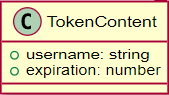
\includegraphics[width=4.5cm]{classes/auth/4.png}}
\end{wrapfigure} 
\par
This class depicts a unencrypted access token.
\newline
\newline
\textbf{Attributes}
\begin{itemize}
    \item \textbf{username} username of the owner of the token
    \item \textbf{expiration} expiration time of the token
\end{itemize}

\subsection{Workspace Management}

\subsubsection{WorkspaceModel}
\label{WorkspaceModel}
\begin{wrapfigure}{l}{4.5cm}
    \raisebox{0pt}[\dimexpr\height-0.5\baselineskip\relax]{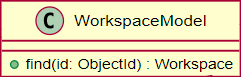
\includegraphics[width=4.5cm]{classes/workspace-management/1.png}}
\end{wrapfigure} 
\par
The collection of workspaces in the database.
\newline
\newline
\textbf{Methods}
\begin{itemize}
    \item \textbf{find} returns the workspace with the given ID.
\end{itemize}

\subsubsection{Workspace}
\label{wm-Workspace}
\begin{wrapfigure}{l}{4.5cm}
    \raisebox{0pt}[\dimexpr\height-0.5\baselineskip\relax]{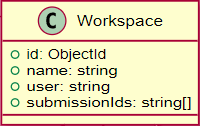
\includegraphics[width=4.5cm]{classes/workspace-management/2.png}}
\end{wrapfigure} 
\par
The document that includes all the relevant information about a workspace.
\newline
\newline
\textbf{Attributes}
\begin{itemize}
    \item \textbf{name} name of the workspace
    \item \textbf{user} user of the workspace
    \item \textbf{submissionIds} all valid submission IDs of the workspace
\end{itemize}

\subsubsection{SensorType}
\label{SensorType}
\begin{wrapfigure}{l}{4.5cm}
    \raisebox{0pt}[\dimexpr\height-0.5\baselineskip\relax]{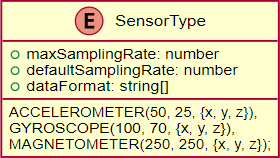
\includegraphics[width=4.5cm]{classes/workspace-management/4.png}}
\end{wrapfigure} 
\par
This enumeration consists of the supported sensors.
\newline
\newline
\textbf{Attributes}
\begin{itemize}
    \item \textbf{maxSamplingRate} the maximum sampling rate of the sensor
    \item \textbf{defaultSamplingRate} the default sampling rate of the sensor
    \item \textbf{dataFormat} the data format of the sensor
\end{itemize}

\subsubsection{Sensor}
\label{Sensor}
\begin{wrapfigure}{l}{4.5cm}
    \raisebox{0pt}[\dimexpr\height-0.5\baselineskip\relax]{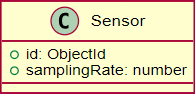
\includegraphics[width=4.5cm]{classes/workspace-management/3.png}}
\end{wrapfigure} 
\par
This class represents a chosen sensor of the workspace. 
\newline
\newline

\textbf{Attributes}
\begin{itemize}
    \item \textbf{samplingRate} the selected sampling rate of the sensor
\end{itemize}

\subsubsection{Label}
\label{Label}
\begin{wrapfigure}{l}{4.5cm}
    \raisebox{0pt}[\dimexpr\height-0.5\baselineskip\relax]{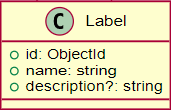
\includegraphics[width=4.5cm]{classes/workspace-management/5.png}}
\end{wrapfigure} 
\par
This class represent an action that describes a sample.
\newline
\newline
\textbf{Attributes}
\begin{itemize}
    \item \textbf{name} name of the label
    \item \textbf{description} description of the label
\end{itemize}

\subsubsection{SampleModel}
\label{SampleModel}
\begin{wrapfigure}{l}{4.5cm}
    \raisebox{0pt}[\dimexpr\height-0.5\baselineskip\relax]{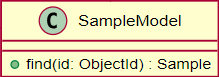
\includegraphics[width=4.5cm]{classes/workspace-management/6.png}}
\end{wrapfigure} 
\par
The collection of samples in the database.
\newline
\newline
\textbf{Methods}
\begin{itemize}
    \item \textbf{find} returns the sample with the given ID.
\end{itemize}

\subsubsection{Sample}
\label{Sample}
\begin{wrapfigure}{l}{4.5cm}
    \raisebox{0pt}[\dimexpr\height-0.5\baselineskip\relax]{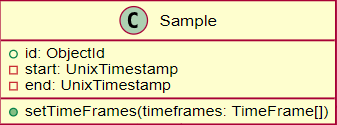
\includegraphics[width=4.5cm]{classes/workspace-management/7.png}}
\end{wrapfigure} 
\par
This class represents a document in the database that contains raw sensor data, its selected timeframes and its label.
\newline
\newline
\textbf{Attributes}
\begin{itemize}
    \item \textbf{start} the timestamp of the start of recording
    \item \textbf{end} the timestamp of the end of recording
\end{itemize}
\textbf{Methods}
\begin{itemize}
    \item \textbf{setTimeFrames} sets the timeframes of the sample
\end{itemize}

\subsubsection{SensorDataPoints}
\label{SensorDataPoints}
\begin{wrapfigure}{l}{4.5cm}
    \raisebox{0pt}[\dimexpr\height-0.5\baselineskip\relax]{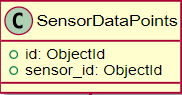
\includegraphics[width=4.5cm]{classes/workspace-management/8.png}}
\end{wrapfigure} 
\par
This class represents data points of a specific sensor.
\newline
\newline
\textbf{Attributes}
\begin{itemize}
    \item \textbf{sensor\_id} the ID of the sensor to which the data belongs
\end{itemize}

\subsubsection{DataPoint}
\label{DataPoint}
\begin{wrapfigure}{l}{4.5cm}
    \raisebox{0pt}[\dimexpr\height-0.5\baselineskip\relax]{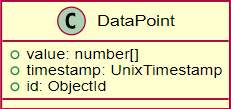
\includegraphics[width=4.5cm]{classes/workspace-management/9.png}}
\end{wrapfigure} 
\par
This class holds the values of a specific sensor at a specific timestamp.
\newline
\newline
\textbf{Attributes}
\begin{itemize}
    \item \textbf{value} the values of the sensor at the specified time
    \item \textbf{timestamp} the timestamp of the sensor values
\end{itemize}

\subsubsection{TimeFrame}
\label{TimeFrame}
\begin{wrapfigure}{l}{4.5cm}
    \raisebox{0pt}[\dimexpr\height-0.5\baselineskip\relax]{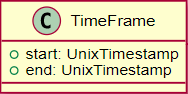
\includegraphics[width=4.5cm]{classes/workspace-management/10.png}}
\end{wrapfigure} 
\par
This class represents a timeframe, which describes a valid intervall of a recorded sample. By setting the wished timeframes, the user can discard parts of a recording.
\newline
\newline
\textbf{Attributes}
\begin{itemize}
    \item \textbf{start} start of the timeframe
    \item \textbf{end} end of the timeframe
\end{itemize}

\subsection{Model Management}

\subsubsection{Trainer}
\label{Trainer}
\begin{wrapfigure}{l}{4.5cm}
    \raisebox{0pt}[\dimexpr\height-0.5\baselineskip\relax]{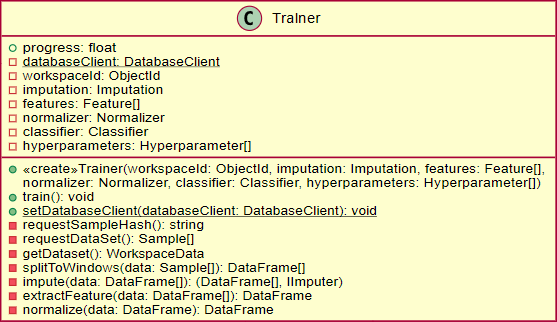
\includegraphics[width=4.5cm]{classes/model-management/1.png}}
\end{wrapfigure} 
\par
Objects of this class performs a machine learning model training process. A new instance is created with each model training. The raw data is fetched from the workspace management service if it is not already present in the local database. The data preprocessing steps are performed before the training and are stored in the local database. For the compatible parameters, the processed data is fetched directly from the database for training. The detailed functioning of the class can be found in the corresponding sequence diagram. The model is saved to the database of the server once the training concludes.
\newline
\newline
\textbf{Attributes}
\begin{itemize}
    \item \textbf{progress} the progress of the training in percent
    \item \textbf{databaseClient} the database client the class uses for database communication
    \item \textbf{workspaceId} the id of the workspace that the training takes place on
    \item \textbf{imputation} the imputation method of the training
    \item \textbf{features} the features to be extracted
    \item \textbf{normalizer} the normalization method of the training
    \item \textbf{classifier} the classifier of the training
    \item \textbf{hyperparameters} the hyperparameters of the classifier as well as the window sizes for the sliding window process
\end{itemize}
\textbf{Methods}
\begin{itemize}
    \item \textbf{train} the method that initiates the model training
    \item \textbf{setDatabaseClient} the static method that sets the database client for the class
    \item \textbf{requestSampleHash} the method that asks the workspace management server for the hash of the samples of the workspace. If the hash is same as the one stored in the local database, samples are directly used from the local database and fetched from the external service otherwise.
    \item \textbf{requestDataSet} the method that requests the data set of the workspace
    \item \textbf{splitToWindows} the method that splits the data set into windows according to the hyper parameters. This method uses the available data from the database if the same computation is already performed before.
    \item \textbf{impute} the method that imputes the training data according to the selected imputation method. This method uses the available data form the database if the same computation is already performed before.
    \item \textbf{extractFeature} this method extracts the features for the training. If a feature with compatible parameters are extracted before, the stored data is used instead of extracting them again.
    \item \textbf{normalize} this method normalizes the data with the specified normalization method
\end{itemize}

\subsubsection{Workspace}
\label{mm-Workspace}
\begin{wrapfigure}{l}{4.5cm}
    \raisebox{0pt}[\dimexpr\height-0.5\baselineskip\relax]{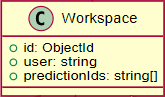
\includegraphics[width=4.5cm]{classes/model-management/2.png}}
\end{wrapfigure} 
\par
The document that includes all the relevant information about a workspace.
\newline
\newline
\textbf{Attributes}
\begin{itemize}
    \item \textbf{user} the user of the workspace
    \item \textbf{predictionIds} the generated prediction ids belonging to the workspace
\end{itemize}

\subsubsection{Sensor}
\label{mm-Sensor}
\begin{wrapfigure}{l}{4.5cm}
    \raisebox{0pt}[\dimexpr\height-0.5\baselineskip\relax]{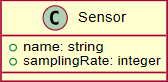
\includegraphics[width=4.5cm]{classes/model-management/3.png}}
\end{wrapfigure} 
\par
The class represents a sensor of the workspace with its sampling rate.
\newline
\newline
\textbf{Attributes}
\begin{itemize}
    \item textbf{name} name of the sensor
    \item textbf{samplingRate} sampling rate of the sensor
\end{itemize}

\subsubsection{MLModel}
\label{MLModel}
\begin{wrapfigure}{l}{4.5cm}
    \raisebox{0pt}[\dimexpr\height-0.5\baselineskip\relax]{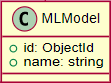
\includegraphics[width=4.5cm]{classes/model-management/4.png}}
\end{wrapfigure} 
\par
This document stores all the relevant information about a trained machine learning model.
\newline
\newline
\textbf{Attributes}
\begin{itemize}
    \item \textbf{name} the name of the model
\end{itemize}

\subsubsection{Imputation}
\label{Imputation}
\begin{wrapfigure}{l}{4.5cm}
    \raisebox{0pt}[\dimexpr\height-0.5\baselineskip\relax]{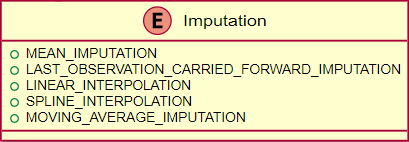
\includegraphics[width=4.5cm]{classes/model-management/5.png}}
\end{wrapfigure} 
\par
This enumeration includes all the available imputation methods.
\newline
\newline

\subsubsection{Feature}
\label{Feature}
\begin{wrapfigure}{l}{4.5cm}
    \raisebox{0pt}[\dimexpr\height-0.5\baselineskip\relax]{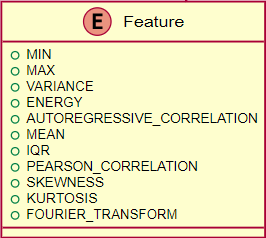
\includegraphics[width=4.5cm]{classes/model-management/6.png}}
\end{wrapfigure} 
\par
This enumeration includes all the available features to extract.
\newline
\newline

\subsubsection{Normalizer}
\label{Normalizer}
\begin{wrapfigure}{l}{4.5cm}
    \raisebox{0pt}[\dimexpr\height-0.5\baselineskip\relax]{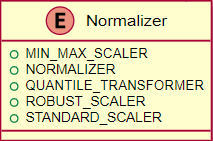
\includegraphics[width=4.5cm]{classes/model-management/7.png}}
\end{wrapfigure} 
\par
This enumeration includes all the normalization methods to use.
\newline
\newline

\subsubsection{Factory}
\label{Factory}
\begin{wrapfigure}{l}{4.5cm}
    \raisebox{0pt}[\dimexpr\height-0.5\baselineskip\relax]{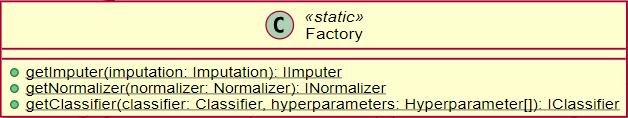
\includegraphics[width=4.5cm]{classes/model-management/8.png}}
\end{wrapfigure} 
\par
This static class is responsible for creating imputer, normalizer and classifier objects.
\newline
\newline
\textbf{Methods}
\begin{itemize}
    \item \textbf{getImputer} creates and returns an imputer object with the given name of the imputer
    \item \textbf{getNormalizer} creates and returns a normalizer object with the given name of the normalizer
    \item \textbf{getClassifier} creates and returns a classifier object with the given name of the classifier
\end{itemize}

\subsubsection{IImputer}
\label{IImputer}
\begin{wrapfigure}{l}{4.5cm}
    \raisebox{0pt}[\dimexpr\height-0.5\baselineskip\relax]{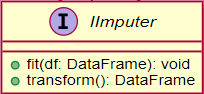
\includegraphics[width=4.5cm]{classes/model-management/9.png}}
\end{wrapfigure} 
\par
This is an interface for an imputer object.
\newline
\newline
\textbf{Methods}
\begin{itemize}
    \item \textbf{fit} fits the given data in the imputer object
    \item \textbf{transform} imputes the given data
\end{itemize}

\subsubsection{INormalizer}
\label{INormalizer}
\begin{wrapfigure}{l}{4.5cm}
    \raisebox{0pt}[\dimexpr\height-0.5\baselineskip\relax]{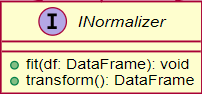
\includegraphics[width=4.5cm]{classes/model-management/10.png}}
\end{wrapfigure} 
\par
This is an interface for a normalizer object.
\newline
\newline
\textbf{Methods}
\begin{itemize}
    \item \textbf{fit} fits the given data in the normalizer object
    \item \textbf{transform} normalizes the given data
\end{itemize}

\subsubsection{IClassifier}
\label{IClassifier}
\begin{wrapfigure}{l}{4.5cm}
    \raisebox{0pt}[\dimexpr\height-0.5\baselineskip\relax]{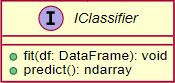
\includegraphics[width=4.5cm]{classes/model-management/11.png}}
\end{wrapfigure} 
\par
This is an interface for a classifier object.
\newline
\newline
\textbf{Methods}
\begin{itemize}
    \item \textbf{fit} fits the given data in the classifier object
    \item \textbf{predict} predicts of which label this data is
\end{itemize}

\subsubsection{PerfomanceMetrics}
\label{PerformanceMetrics}
\begin{wrapfigure}{l}{4.5cm}
    \raisebox{0pt}[\dimexpr\height-0.5\baselineskip\relax]{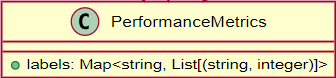
\includegraphics[width=4.5cm]{classes/model-management/12.png}}
\end{wrapfigure} 
\par
This class represents the performance metrics of a trained model.
\newline
\newline
\textbf{Attributes}
\begin{itemize}
    \item \textbf{labels} map of labels to their performance metrics
\end{itemize}

\subsubsection{Hyperparameter}
\label{Hyperparameter}
\begin{wrapfigure}{l}{4.5cm}
    \raisebox{0pt}[\dimexpr\height-0.5\baselineskip\relax]{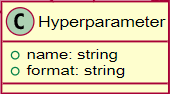
\includegraphics[width=4.5cm]{classes/model-management/13.png}}
\end{wrapfigure} 
\par
This class represents a hyperparameter for training a model.
\newline
\newline
\textbf{Attributes}
\begin{itemize}
    \item \textbf{name} name of the hyperparameter
    \item \textbf{format} the format of the value that the hyperparameter can get
\end{itemize}

\subsubsection{WorkspaceData}
\label{WorkspaceData}
\begin{wrapfigure}{l}{4.5cm}
    \raisebox{0pt}[\dimexpr\height-0.5\baselineskip\relax]{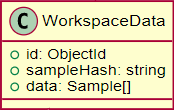
\includegraphics[width=4.5cm]{classes/model-management/14.png}}
\end{wrapfigure} 
\par
This class holds the sample data from the last training.
\newline
\newline
\textbf{Attributes}
\begin{itemize}
    \item \textbf{sampleHash} hash of the sample data
    \item \textbf{data} the sample data
\end{itemize}

\subsubsection{SlidingWindow}
\label{SlidingWindow}
\begin{wrapfigure}{l}{4.5cm}
    \raisebox{0pt}[\dimexpr\height-0.5\baselineskip\relax]{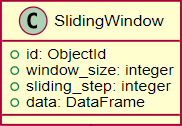
\includegraphics[width=4.5cm]{classes/model-management/15.png}}
\end{wrapfigure} 
\par
This class hold the sample data from recent trainings which is split into windows.
\newline
\newline
\textbf{Attributes}
\begin{itemize}
    \item \textbf{window\_size} size of the windows
    \item \textbf{sliding\_step} the sliding step of the windows
    \item \textbf{data} the sliding windows
\end{itemize}

\subsubsection{ImputedData}
\label{ImputedData}
\begin{wrapfigure}{l}{4.5cm}
    \raisebox{0pt}[\dimexpr\height-0.5\baselineskip\relax]{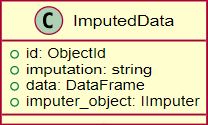
\includegraphics[width=4.5cm]{classes/model-management/16.png}}
\end{wrapfigure} 
\par
This class holds the imputed data from recent trainings.
\newline
\newline
\textbf{Attributes}
\begin{itemize}
    \item \textbf{imputation} the used imputation method
    \item \textbf{data} the imputed data
    \item \textbf{imputer\_object} the used imputer object
\end{itemize}

\subsubsection{ExtractedFeature}
\label{ExtractedFeature}
\begin{wrapfigure}{l}{4.5cm}
    \raisebox{0pt}[\dimexpr\height-0.5\baselineskip\relax]{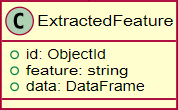
\includegraphics[width=4.5cm]{classes/model-management/17.png}}
\end{wrapfigure} 
\par
This class holds the extracted features of the data from recent trainings.
\newline
\newline
\textbf{Attributes}
\begin{itemize}
    \item \textbf{feature} the extracted feature
    \item \textbf{data} the values of the feature
\end{itemize}
